\documentclass[12pt,a4paper]{report}
\usepackage[utf8]{inputenc}
\usepackage[T1]{fontenc}
\usepackage[french]{babel}
\usepackage{graphicx}
\usepackage{hyperref}
\usepackage{lipsum}  % Pour le texte exemple
\usepackage{makeidx}
\usepackage{tocloft}
\usepackage{xcolor}

% Configuration des liens hypertexte
\hypersetup{
    colorlinks=true,
    linkcolor=blue,
    filecolor=magenta,
    urlcolor=cyan,
}

\makeindex

\begin{document}

% Première page de titre
\begin{titlepage}
\begin{center}
    \vspace*{2cm}
    {\LARGE\textbf{Système de prévision et d’alerte de la pollution atmosphérique}}\\[1cm]
    {\large Par}\\[0.5cm]
    {\large DAOUDI Mohamed Raouf}\\
    {\large et BOUROUIS Abdeldjalil}\\[1cm]
    {\large Mémoire présenté à}\\
    {\large Université d'Alger 1}\\[1cm]
    {\large Pour l'obtention du}\\
    {\large Diplôme de Master}\\[2cm]
    {\large \today}
\end{center}
\end{titlepage}

% Page blanche
\newpage
\thispagestyle{empty}
\mbox{}

% Page de titre répétée
\newpage
\begin{titlepage}
\begin{center}
    \vspace*{2cm}
    {\LARGE\textbf{Système de prévision et d’alerte de la pollution atmosphérique}}\\[1cm]
    {\large Par}\\[0.5cm]
    {\large DAOUDI Mohamed Raouf}\\
    {\large et BOUROUIS Abdeldjalil}\\[1cm]
    {\large Mémoire présenté à}\\
    {\large Université d'Alger 1}\\[1cm]
    {\large Pour l'obtention du}\\
    {\large Diplôme de Master}\\[2cm]
    {\large \today}
\end{center}
\end{titlepage}

% Sommaire
\newpage
\phantomsection
\addcontentsline{toc}{chapter}{SOMMAIRE}
\chapter*{SOMMAIRE}
\tableofcontents

% Table des illustrations
\newpage
\phantomsection
\addcontentsline{toc}{chapter}{TABLE DES ILLUSTRATIONS}
\chapter*{TABLE DES ILLUSTRATIONS}
\listoffigures

% Résumé/Abstract
\newpage
\phantomsection
\addcontentsline{toc}{chapter}{RÉSUMÉ}
\chapter*{RÉSUMÉ}
La pollution atmosphérique constitue une menace majeure pour la santé publique et l’environnement, exacerbée par des facteurs tels que les émissions industrielles, le trafic routier et d’autres activités anthropiques. Ce travail de recherche propose la conception et le développement d’un système de prévision et d’alerte de la pollution atmosphérique utilisant des techniques d’apprentissage profond. Ce système vise à exploiter de grandes quantités de données environnementales pour identifier des schémas complexes et fournir des prévisions précises en temps réel. Le projet inclut une revue des approches existantes, la conception d’une architecture intégrant des modèles avancés, le développement d’un système d’alerte pour informer les utilisateurs, et une évaluation des performances des modèles prédictifs. L’objectif est de contribuer à la réduction des impacts sanitaires et environnementaux liés à la pollution de l’air en proposant une solution technologique innovante.

% Page blanche avant introduction
\newpage
\thispagestyle{empty}
\begin{center}
\vspace*{\fill}
{\Huge\textbf{INTRODUCTION}}
\vspace*{\fill}
\end{center}

% Introduction
\chapter{INTRODUCTION}
La pollution atmosphérique est l’un des défis environnementaux les plus pressants de notre époque. En raison de l’urbanisation croissante, de l’industrialisation et de l’augmentation des activités humaines, les concentrations de polluants atmosphériques, tels que les particules fines (PM2.5 et PM10), l’ozone (O$_3$) et le dioxyde d’azote (NO$_2$), continuent d’atteindre des niveaux préoccupants. Ces polluants sont responsables de nombreuses maladies respiratoires, cardiovasculaires et d’une détérioration significative de la qualité de vie, particulièrement dans les zones urbaines densément peuplées.

Face à ces enjeux, il devient impératif de disposer de systèmes robustes capables de prédire avec précision les épisodes de pollution et d’informer les populations à risque. L’intégration de l’intelligence artificielle, et plus spécifiquement de l’apprentissage profond, ouvre de nouvelles perspectives pour l’analyse de données environnementales complexes et la prévision en temps réel de la qualité de l’air. Les capacités de ces modèles à apprendre et à détecter des motifs subtils permettent de dépasser les limitations des approches traditionnelles.

Dans ce contexte, ce travail de recherche vise à développer un système de prévision et d’alerte de la pollution atmosphérique, en s’appuyant sur des algorithmes d’apprentissage profond pour analyser de grandes quantités de données et générer des alertes précoces. Ce système ambitionne de réduire les impacts sanitaires et environnementaux en permettant une meilleure anticipation des épisodes de pollution et une prise de décision éclairée par les autorités et les citoyens. Les résultats obtenus contribueront à renforcer la lutte contre la pollution atmosphérique en proposant une solution technologique avancée adaptée aux défis actuels.
\subsection{Analyse des sources et impacts de la pollution}
La pollution atmosphérique résulte d'une interaction complexe entre différentes sources, causes et conséquences. Le tableau suivant présente une synthèse des principaux facteurs et leurs impacts :
\begin{figure}[h]
    \centering
    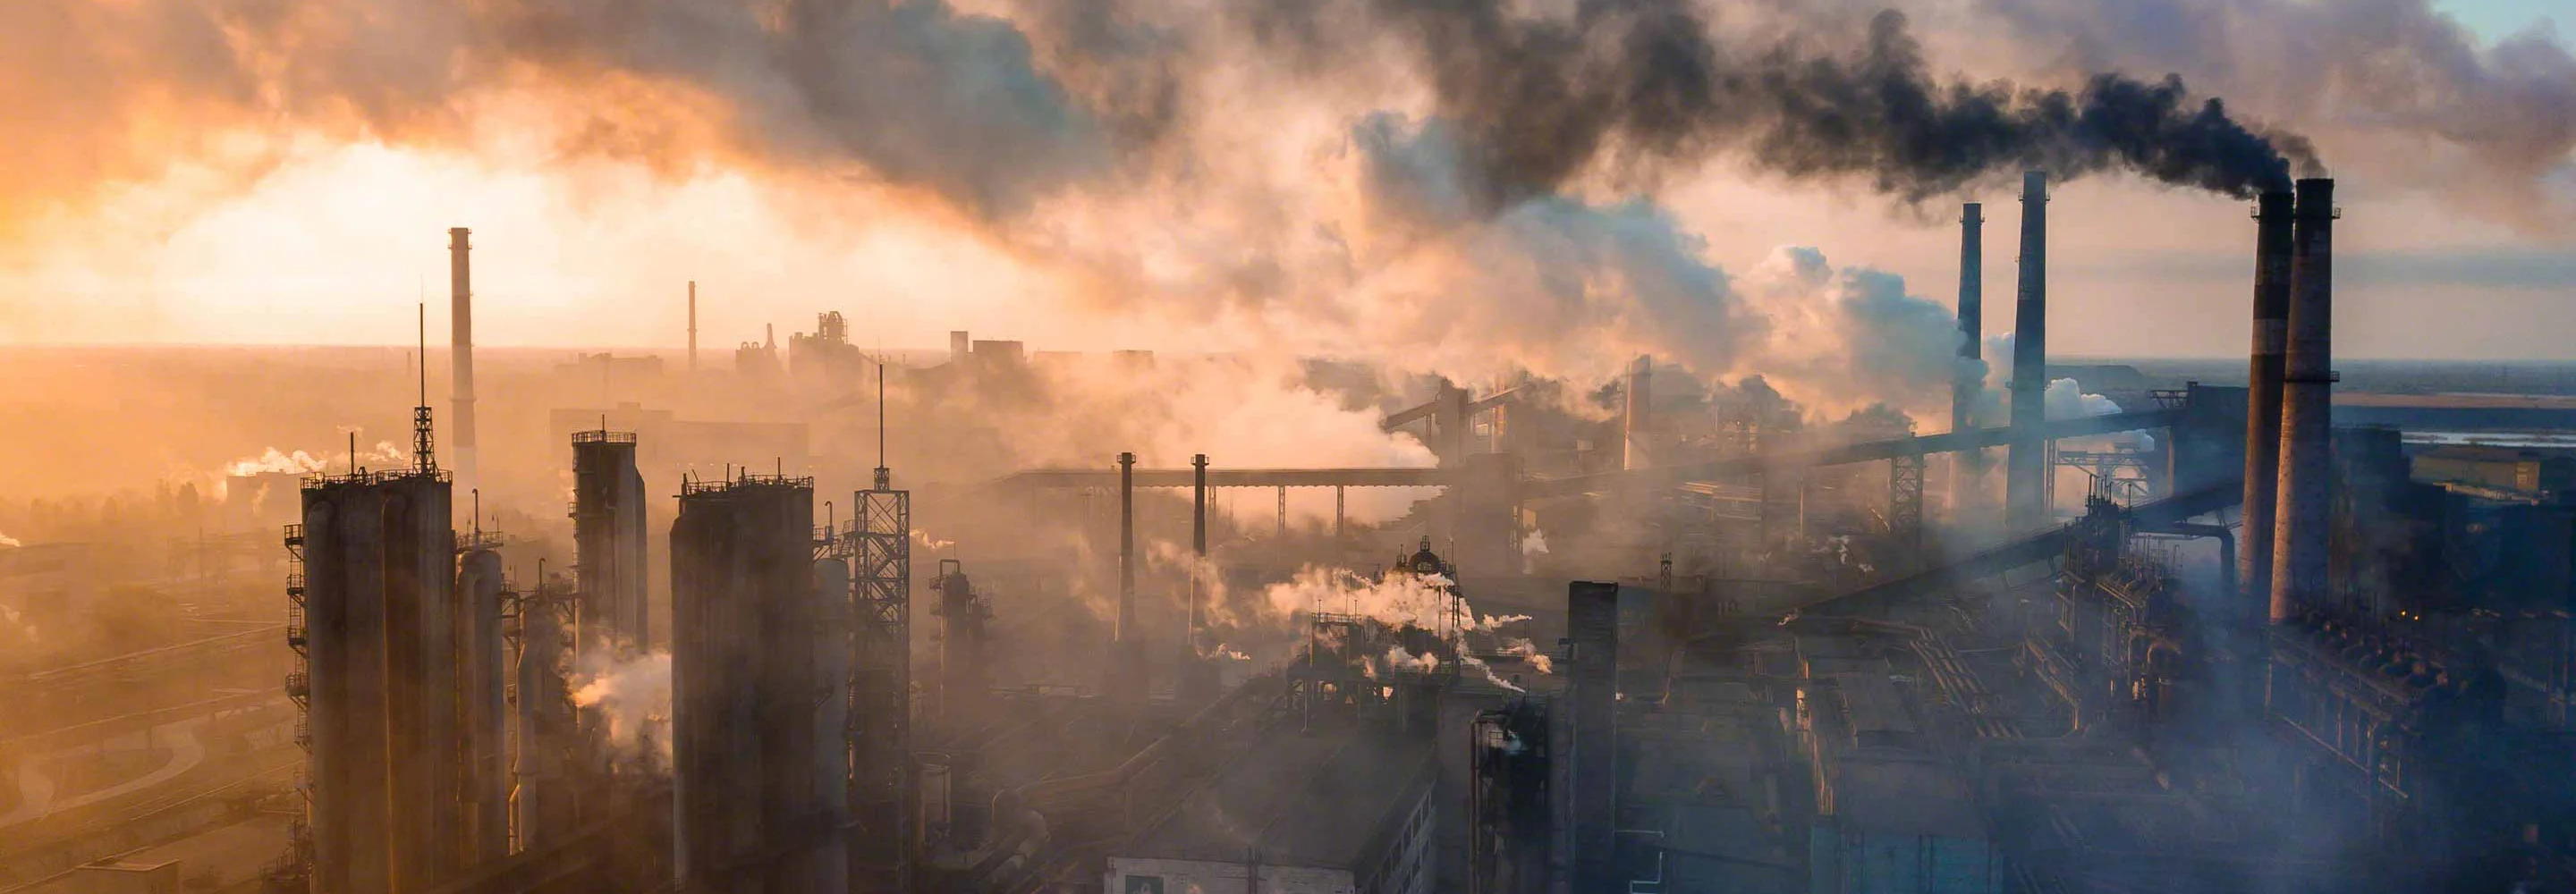
\includegraphics[width=0.8\textwidth]{pollution.png}
    \caption{Pollution}
    \label{fig:Pollution}
\end{figure}

\begin{table}[h]
    \centering
    \begin{tabular}{|p{5cm}|p{5cm}|p{5cm}|}
    \hline
    \textbf{Source} & \textbf{Causes} & \textbf{Conséquences} \\
    \hline
    Zones industrielles & Émissions de gaz toxiques & Maladies respiratoires chroniques \\
    \hline
    Zones urbaines & Trafic routier intense & Problèmes cardiovasculaires \\
    \hline
    Zones agricoles & Usage excessif de pesticides & Contamination des sols et de l'eau \\
    \hline
    Centrales électriques & Combustion de charbon/pétrole & Pluies acides et smog \\
    \hline
    Zones résidentielles & Chauffage domestique & Pollution de l'air intérieur \\
    \hline
    Zones portuaires & Transport maritime & Pollution côtière et marine \\
    \hline
    Sites miniers & Extraction de minerais & Dégradation des écosystèmes \\
    \hline
    Décharges & Incinération des déchets & Contamination atmosphérique \\
    \hline
    \end{tabular}
    \caption{Sources, causes et conséquences de la pollution atmosphérique}
    \label{tab:pollution}
    \end{table}
\subsection{Intelligence Artificielle et Apprentissage Profond}
L'Intelligence Artificielle (IA), définie par \cite{Russell2010}, est la science qui permet aux machines d'imiter le comportement intelligent humain. L'apprentissage profond, une branche de l'IA, utilise des réseaux de neurones artificiels multicouches définis par l'équation :

\begin{equation}
    h_{\theta}(x) = f(\sum_{i=1}^{n} w_i x_i + b)
\end{equation}

où $f$ représente la fonction d'activation, $w_i$ les poids, $x_i$ les entrées et $b$ le biais \cite{Goodfellow2016}.
\subsection{Applications de l'IA et de l'Apprentissage Profond}
Les domaines d'application de l'IA et de l'apprentissage profond sont vastes et incluent notamment :
\begin{itemize}
    \item La vision par ordinateur avec les réseaux CNN \cite{LeCun2015}
    \item Le traitement du langage naturel via les architectures Transformer
    \item L'analyse prédictive des séries temporelles
    \item La détection d'anomalies environnementales
\end{itemize}

Dans le contexte de la pollution atmosphérique, ces technologies permettent d'établir des modèles prédictifs complexes exprimés par :

\begin{equation}
    P(t+1) = F(P(t), M(t), E(t))
\end{equation}

où $P(t)$ représente le niveau de pollution au temps $t$, $M(t)$ les conditions météorologiques et $E(t)$ les facteurs environnementaux \cite{Zhang2020}.



% Développement
\chapter{LE REVUE DE LITTÉRATURES}
La prévision de la qualité de l'air est devenue de plus en plus importante dans le contexte de l'urbanisation et de l'industrialisation, compte tenu de son impact sur la santé humaine et la durabilité environnementale. Une étude explorée dans ce domaine a proposé un modèle de prévision de l'indice de qualité de l'air (IQA) basé sur les villes intelligentes qui intègre des techniques de calcul avancées pour une précision améliorée (Author et al., Year). Cette recherche a spécifiquement utilisé un algorithme de régression combiné à des réseaux antagonistes génératifs profonds (GAN) pour le prétraitement et l'imputation des données manquantes dans un ensemble de données sur la qualité de l'air des villes indiennes couvrant la période 2015-2020. L'algorithme a incorporé un GRU Stacked Attention modifié avec divergence KL pour améliorer les capacités de prédiction.

La méthodologie innovante de l'étude, y compris l'utilisation de la mise à l'échelle des caractéristiques et de l'analyse de régression, a relevé efficacement des défis tels que la perte de données et l'imprécision courantes dans les techniques traditionnelles de prévision de l'IQA. Le modèle a démontré des performances supérieures avec des mesures telles que MAE (0,1013), MSE (0,0134) et R² (0,9479), surpassant les algorithmes de régression existants en termes de minimisation des pertes. Des villes comme Ernakulam, Chennai et Ahmedabad ont été présentées comme des études de cas, présentant des niveaux d'AQI élevés, moyens et faibles, respectivement.

Ce travail contribue de manière significative à la littérature en comblant les lacunes des méthodes de prédiction d'AQI existantes, notamment en termes de prétraitement des données et d'optimisation des algorithmes. Cependant, l'étude se concentre principalement sur les villes indiennes, ce qui suggère une limitation potentielle de sa généralisabilité à d'autres régions géographiques avec des profils de polluants et des facteurs environnementaux différents. Néanmoins, ses résultats soulignent l'importance d'intégrer des approches informatiques avancées comme les Deep GAN dans les systèmes de surveillance environnementale, fournissant une référence pour les recherches futures dans le domaine.

\begin{figure}[h]
    \centering
    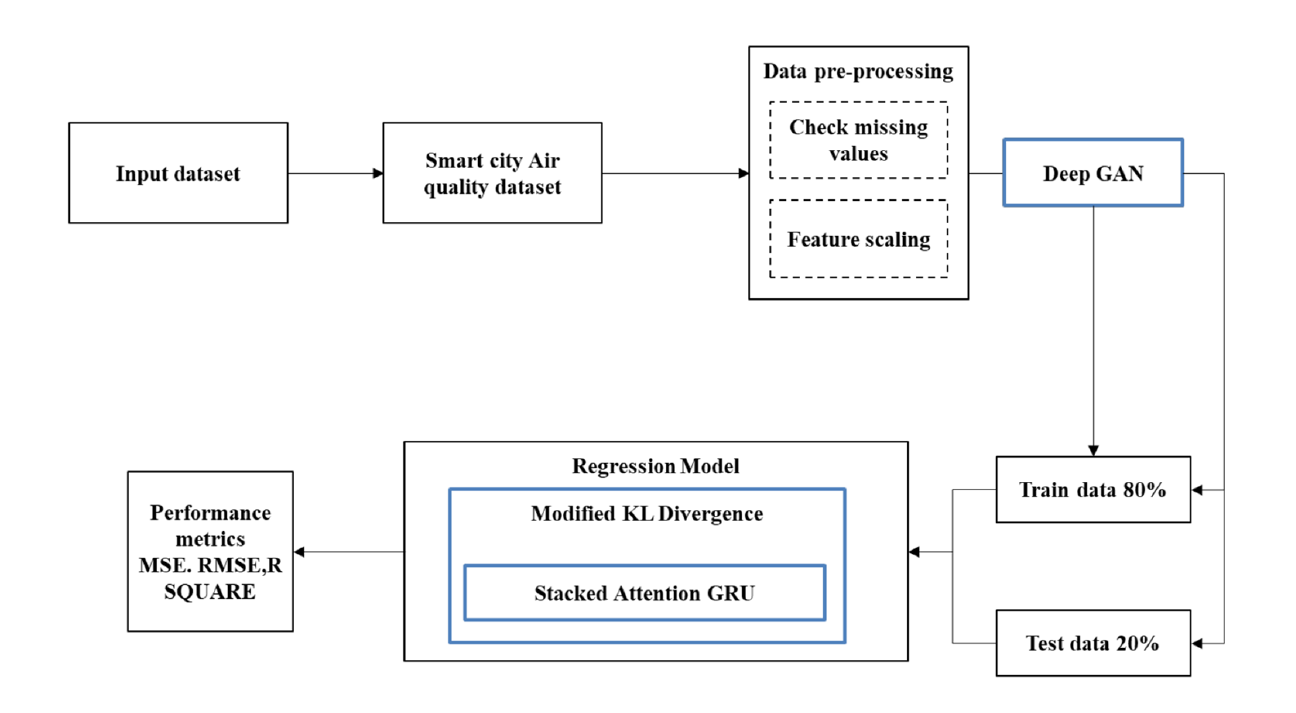
\includegraphics[width=0.8\textwidth]{diagram1.png}
    \caption{Diagram proposé par BINBUSAYYIS}
    \label{fig:Diagram}
\end{figure}

\chapter{CONSIDÉRATIONS MÉTHOLOGIQUES}
\lipsum[1-2]

\chapter{LA DISCUSSION DES RÉSULTATS}
\lipsum[3-4]

% Conclusion
\newpage
\thispagestyle{empty}
\begin{center}
\vspace*{\fill}
{\Huge\textbf{CONCLUSION}}
\vspace*{\fill}
\end{center}

\chapter{CONCLUSION}
\lipsum[5-6]

% Liste des sources
\newpage
\phantomsection
\addcontentsline{toc}{chapter}{LISTE DES SOURCES}
\chapter*{LISTE DES SOURCES}
\begin{itemize}
    \item Source 1: \cite{source1}
\end{itemize}

% Index
\newpage
\phantomsection
\addcontentsline{toc}{chapter}{INDEX}
\printindex

% Bibliographie
\newpage
\phantomsection
\addcontentsline{toc}{chapter}{BIBLIOGRAPHIE}
\bibliographystyle{plain}
\bibliography{references}

% Annexes
\appendix
\chapter*{ANNEXES}
\addcontentsline{toc}{chapter}{ANNEXES}
\lipsum[8]

% Page blanche finale
\newpage
\thispagestyle{empty}
\mbox{}

% Résumé final
\newpage
\phantomsection
\addcontentsline{toc}{chapter}{RÉSUMÉ FINAL}
\chapter*{RÉSUMÉ FINAL}
\lipsum[11]

\end{document}
